\documentclass[3p,onecolumn]{elsarticle}

\usepackage{natbib}
\usepackage[version=4]{mhchem}
\usepackage{graphicx}
\journal{Fluid Phase Equilibria}

\bibliographystyle{elsarticle-num}
%%%%%%%%%%%%%%%%%%%%%%%

\begin{document}

\begin{frontmatter}

\title{A molecular dynamics study of the solvation of carbon dioxide and other compounds in the ionic liquids \ce{[emim][B(CN)_4]} and \ce{[emim][NTf_2]}}

%% Group authors per affiliation:
\author[plapiqui]{A.J.~Silveira\corref{curradd}}
\author[plapiqui]{S.~Pereda}
\author[eq-ufrj,coppe-ufrj]{F.W.~Tavares}
\author[eq-ufrj]{C.R.A.~Abreu\corref{cor1}}
\ead{abreu@eq.ufrj.br}

\address[plapiqui]{Planta Piloto de Ingenier\'ia Qu\'imica (PLAPIQUI), Universidad Nacional del Sur, Bah\'ia Blanca, Argentina}
\address[eq-ufrj]{Chemical Engineering Department, Escola de Qu\'imica, Universidade Federal do Rio de Janeiro, Rio de Janeiro, Brazil}
\address[coppe-ufrj]{Chemical Engineering Program, Alberto Luiz Coimbra Institute for Graduate Studies and Research in Engineering (COPPE), Universidade Federal do Rio de Janeiro, Rio de Janeiro, Brazil}

\cortext[curradd]{Current address: Computational \& Systems Biology Program, Memorial Sloan Kettering Cancer Center, New York, NY, USA}
\cortext[cor1]{Corresponding author}

\end{frontmatter}

\begin{figure}[ht]
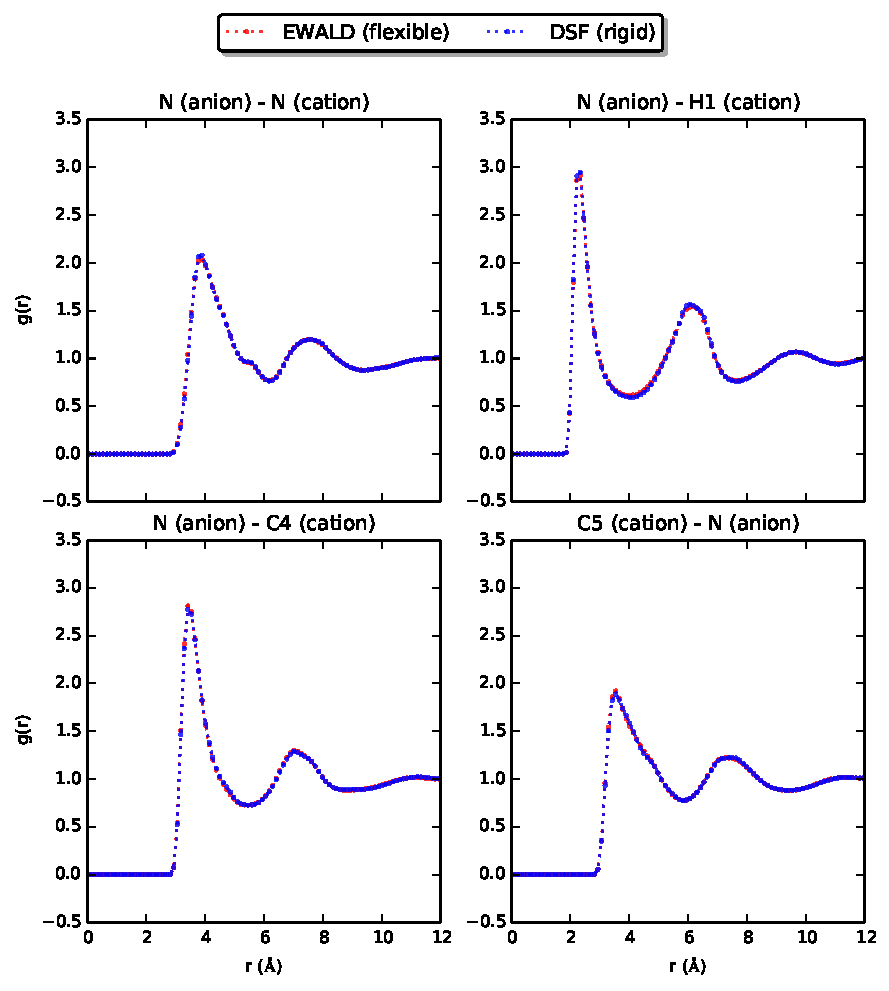
\includegraphics[]{rdf-koller}
\caption{Radial distribution functions $g(r)$ obtained in NPT-MD simulations of 250 ion pairs of \ce{[emim][B(CN)4]} at $T = 298.0~\mathrm{K}$ and $P = 1.0~\mathrm{bar}$ using the model of Koller \textit{et al}. \cite{Koller_2012}.}
\label{fig:rdf-koller}
\end{figure}

\begin{figure}[ht]
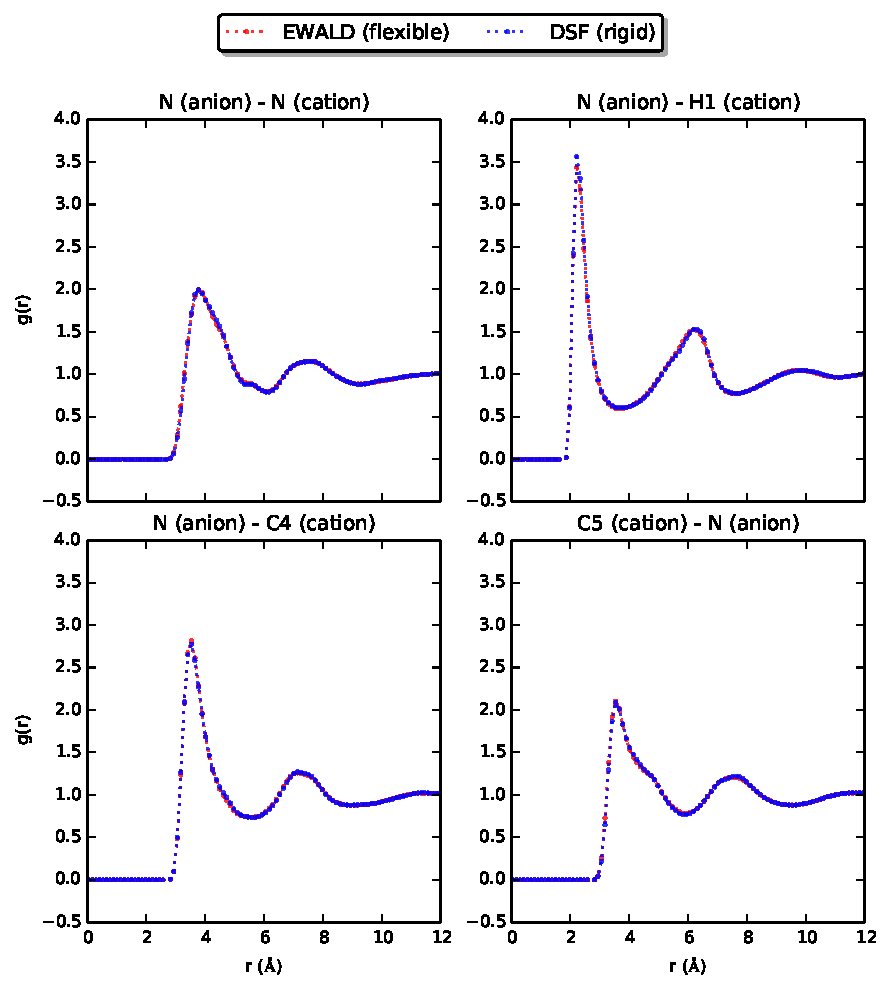
\includegraphics[]{rdf-Batista}
\caption{Radial distribution functions $g(r)$ obtained in NPT-MD simulations of 250 ion pairs of \ce{[emim][B(CN)4]} at $T = 298.0~\mathrm{K}$ and $P = 1.0~\mathrm{bar}$ using the model of Batista \textit{et al}. \cite{Batista_2015}.}
\label{fig:rdf-Batista}
\end{figure}


\begin{figure}[ht]
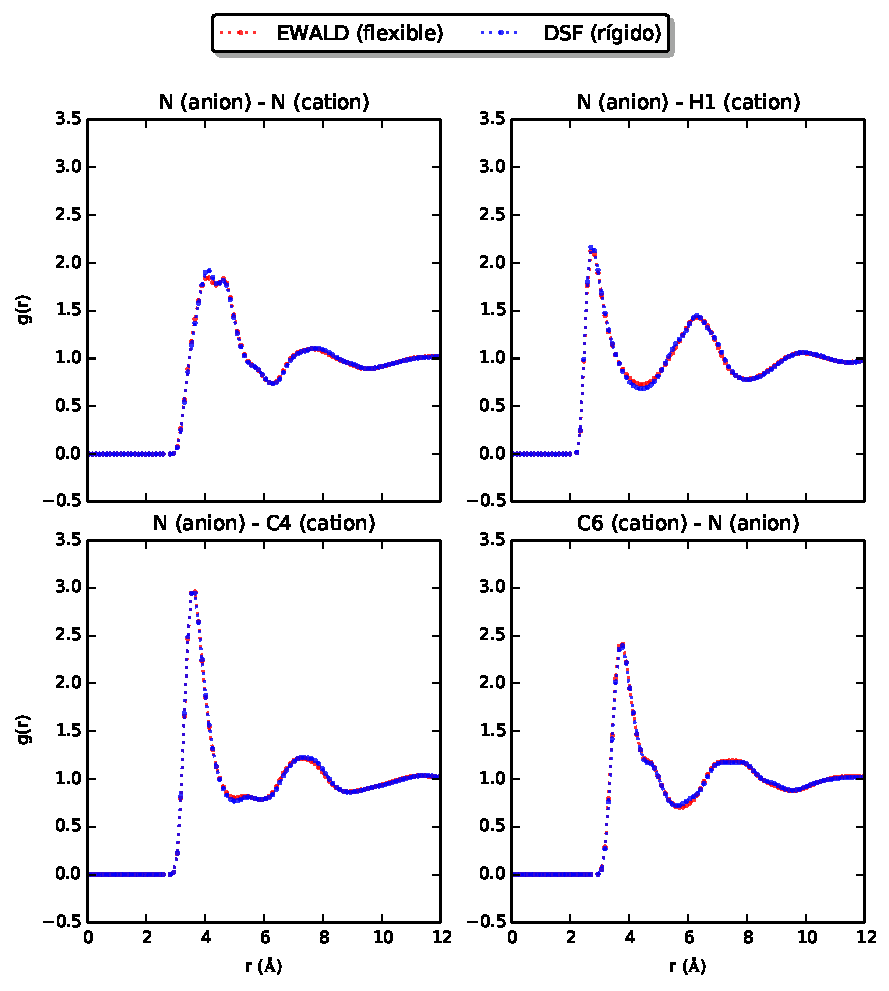
\includegraphics[]{rdf-Liu}
\caption{Radial distribution functions $g(r)$ obtained in NPT-MD simulations of 250 ion pairs of \ce{[emim][B(CN)4]} at $T = 298.0~\mathrm{K}$ and $P = 1.0~\mathrm{bar}$ using the model of Liu \textit{et al}. \cite{Liu_2014}.}
\label{fig:rdf-Liu}
\end{figure}

\begin{figure}[ht]
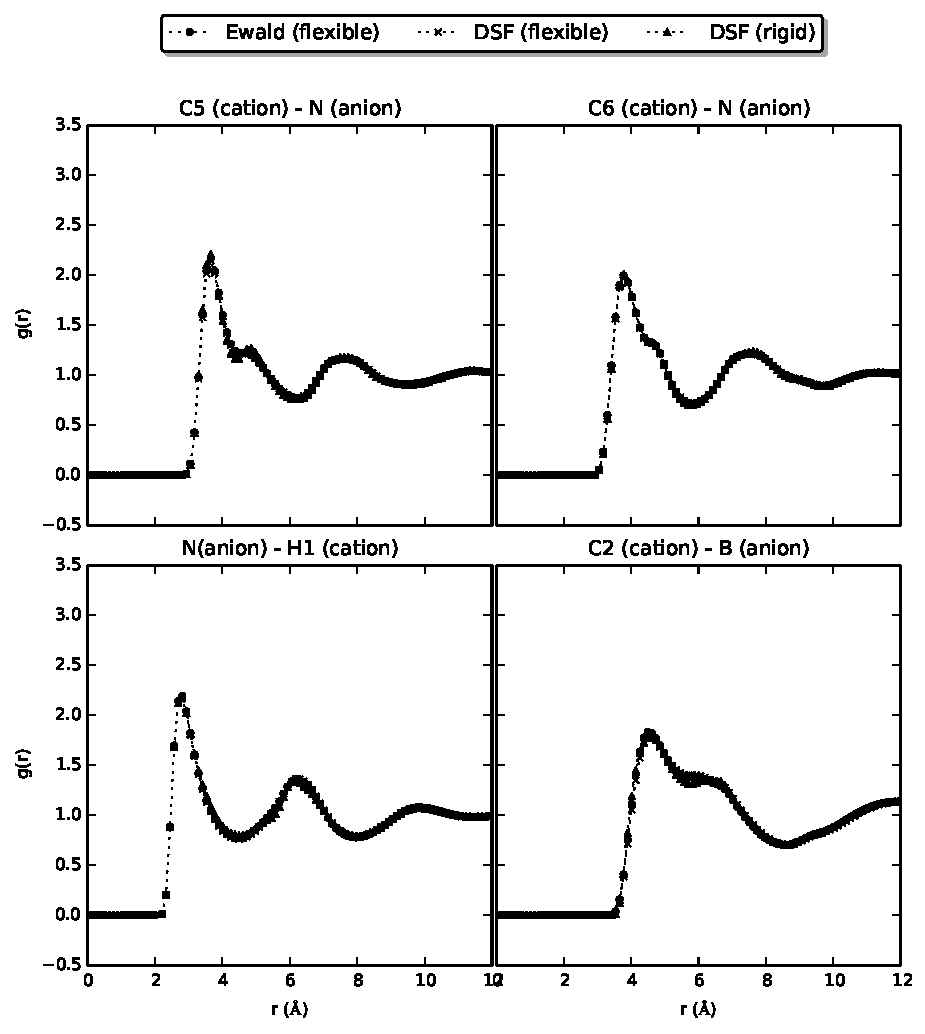
\includegraphics[]{rdf-Weber}
\caption{Radial distribution functions $g(r)$ obtained in NPT-MD simulations of 250 ion pairs of \ce{[emim][B(CN)4]} at $T = 298.0~\mathrm{K}$ and $P = 1.0~\mathrm{bar}$ using the model of Weber and Kirchner \cite{Weber_2016}.}
\label{fig:rdf-Weber}
\end{figure}

\begin{figure}
	\centering
	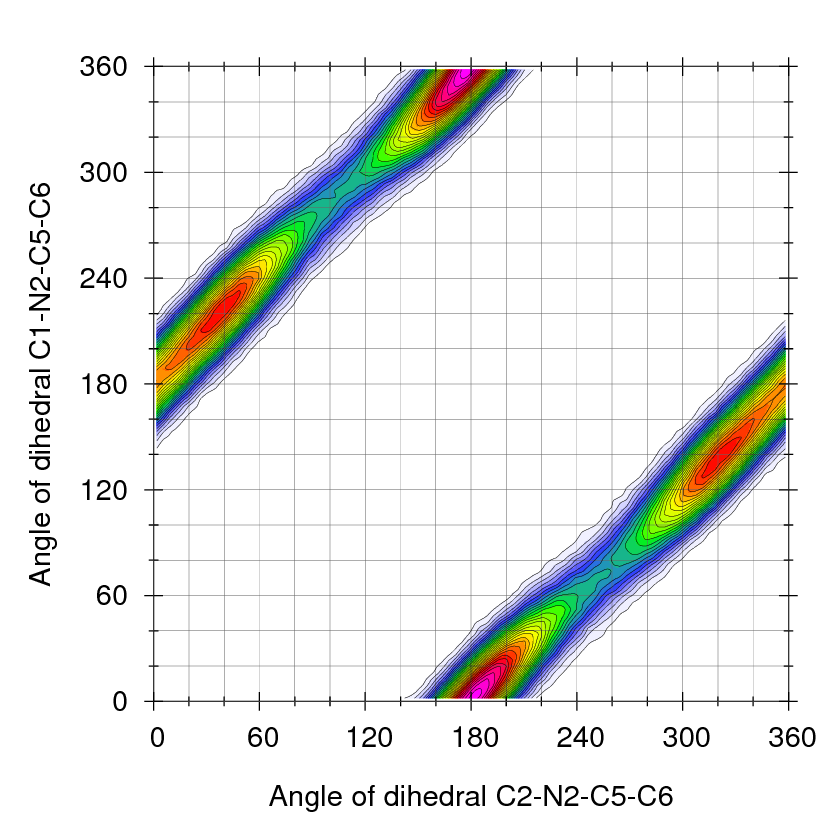
\includegraphics[width=\linewidth]{Ludwig}%
	
	%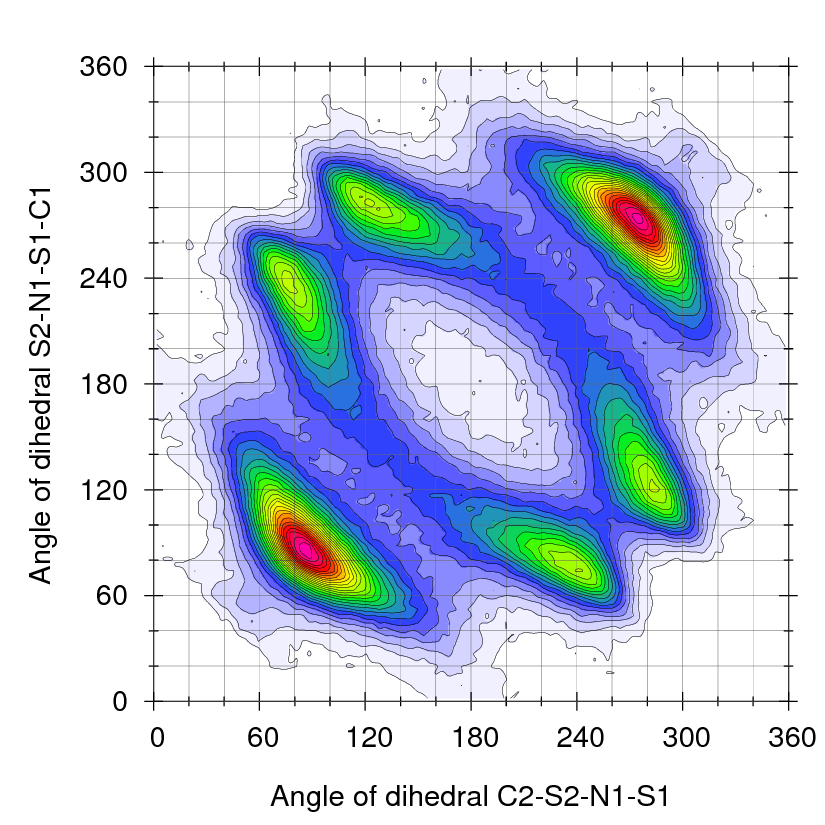
\includegraphics[width=\linewidth]{Ludwig_anion}%
	\caption{Combined distribution function of the dihedral angles of C1-N2-C5-C6 and C2-N2-C5-C6 obtained from NPT-MD simulations of 250 ion pairs of \ce{[emim][NTf_2]} at $T = 298.0~\mathrm{K}$ and $P = 1.0~\mathrm{bar}$ using the model of K\"{o}ddermann \textit{et al}. \cite{Koddermann_2007}.}
	\label{fig:die_ntf2}
\end{figure}

\bibliography{ionic_liquids}

\end{document}